

History of experiment. Pedro found out about our work via Youtube (insomnia). Asked us about an invariant involving billiard curvatures at the vertices, we found $\sum{k^{2/3}}$ but this is a direct corollary of the sum of cosines. This implied $\sum{1/(d_1 d_2)}$ was invariant. Jair gave the idea to check if the stronger result $\sum{1/d_1}$ was invariant, which it was. This corresponds to the sum of the inverse lengths of ``focal spokes'', or the sum of the lengths of the focal spokes to the inversive polygon, both which are invariant. We then simply tested the perimeter of the inversive polygon which was unexpectedly constant.



The bicentric family is a 1d family of Poncelet N-gons interscribed between two specially-chosen circles \cite[Poncelet's Porism]{mw}. The special case of a family of triangles with fixed incircle and circumcircle was originally studied by Chapple 80 years before Poncelet \cite{odehnal2011-poristic}. Any pair of conics can be sent to a pair of circles via a suitable projective transformation \cite{akopyan2007-conics}. Based on this, in the 1820s Jacobi produced an alternative proof to Poncelet's Great theorem based on simplifications afforded by his elliptic functions over the bicentric family \cite{bos-1987,dragovic11,nash2018-poncelet}.

Referring to
\cref{fig:confocal}, a known fact is that the {\em polar image}\footnote{The polar of a point $P$ with respect to a circle $\C$ centered on $O$ is the line $L$ containing the inversion of $P$ wrt $\C$ and perpendicular to $OP$.} of two circles with respect to either one of their {\em limiting points}\footnote{A pair of circles is associated with a pair of {\em limiting points} $\ell_1,\ell_2$ which are centers of inversion that send the original circles to two distinct pairs of concentric circles \cite[Limiting Points]{mw}.} is a pair of confocal conics with a focus coinciding with the limiting point chosen \cite{akopyan2007-conics} (see \cref{app:polar-pedal}). Conversely, the bicentric family is the polar image of elliptic (or hyperbolic) billiard N-periodics with respect to a focus (see \cref{sec:five-polys}). Recall the latter conserve both perimeter\footnote{Billiard inscribed in hyperbolas conserve {\em signed} perimeter, see \cref{sec:five-polys}.} and Joachimsthal's constant \cite{sergei91}.

\begin{figure}
    \centering
    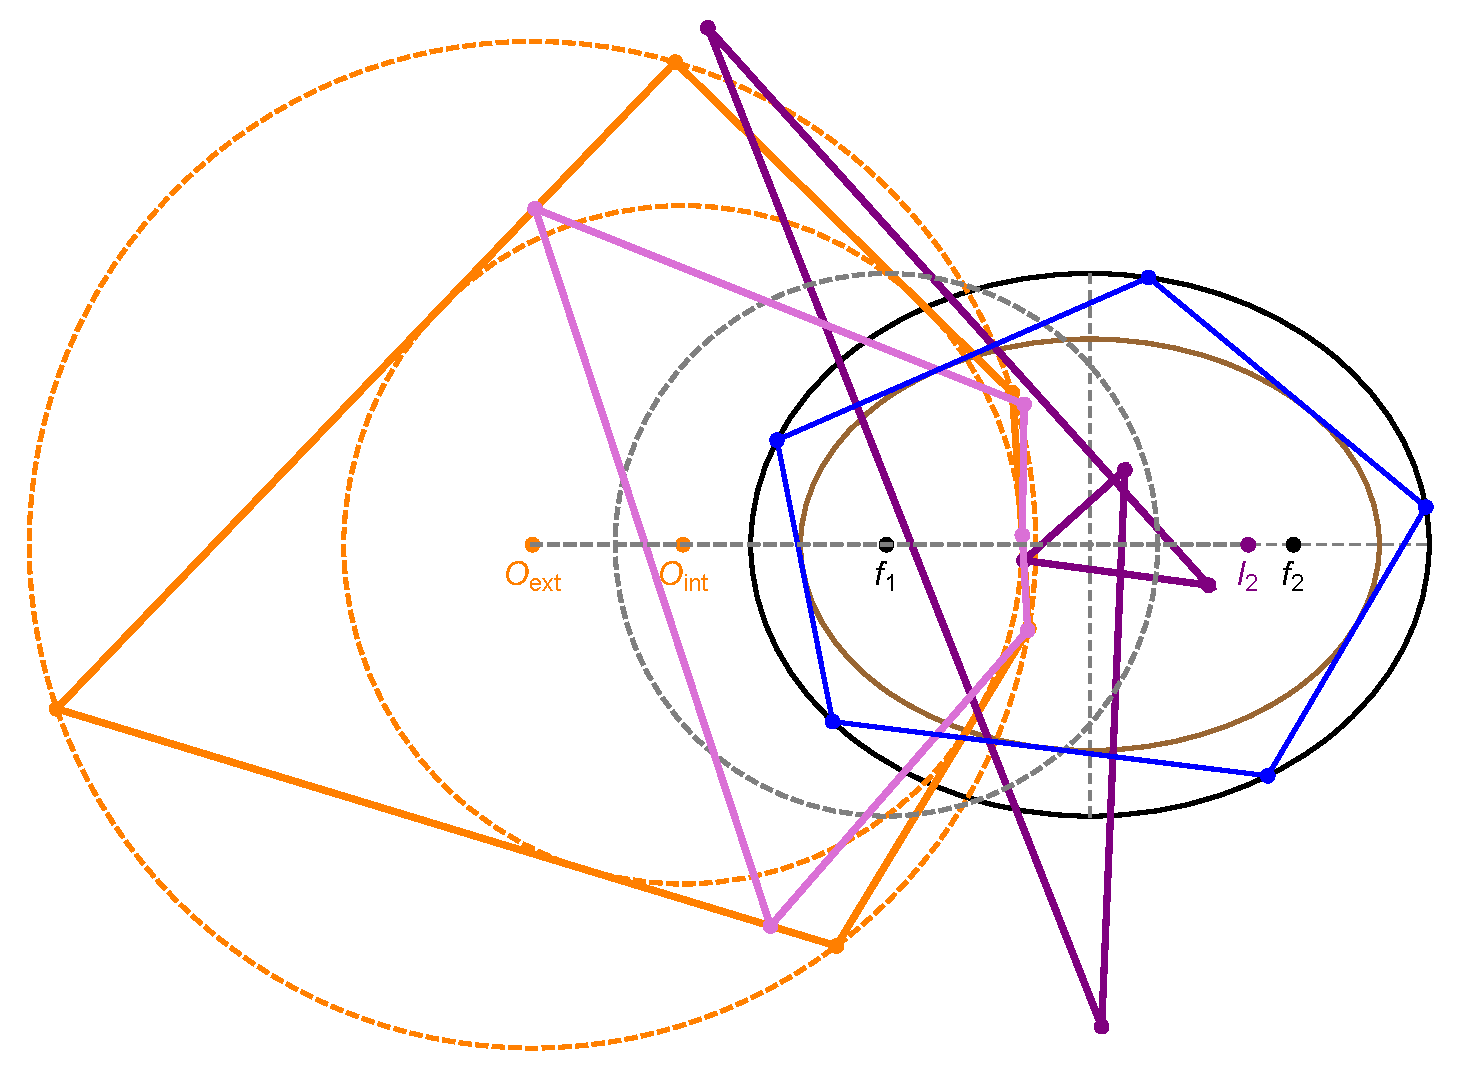
\includegraphics[width=.9\textwidth]{pics_05_0040_billiard_plot.pdf}
    \caption{The bicentric family  (solid orange) is the polar image of elliptic billiard N-periodics (blue) with respect to a circle (dashed gray) centered on $f_1$ (which coincides with limiting point $\ell_1$). Also shown are the constant-perimeter bicentric pedals (pink and purple) with respect to either limiting point, $f_1=\ell_1$ and $\ell_2$.  \href{https://youtu.be/8m21fCz8eX4}{Video}}
    \label{fig:confocal}
\end{figure}

%\begin{figure}
%    \centering
%    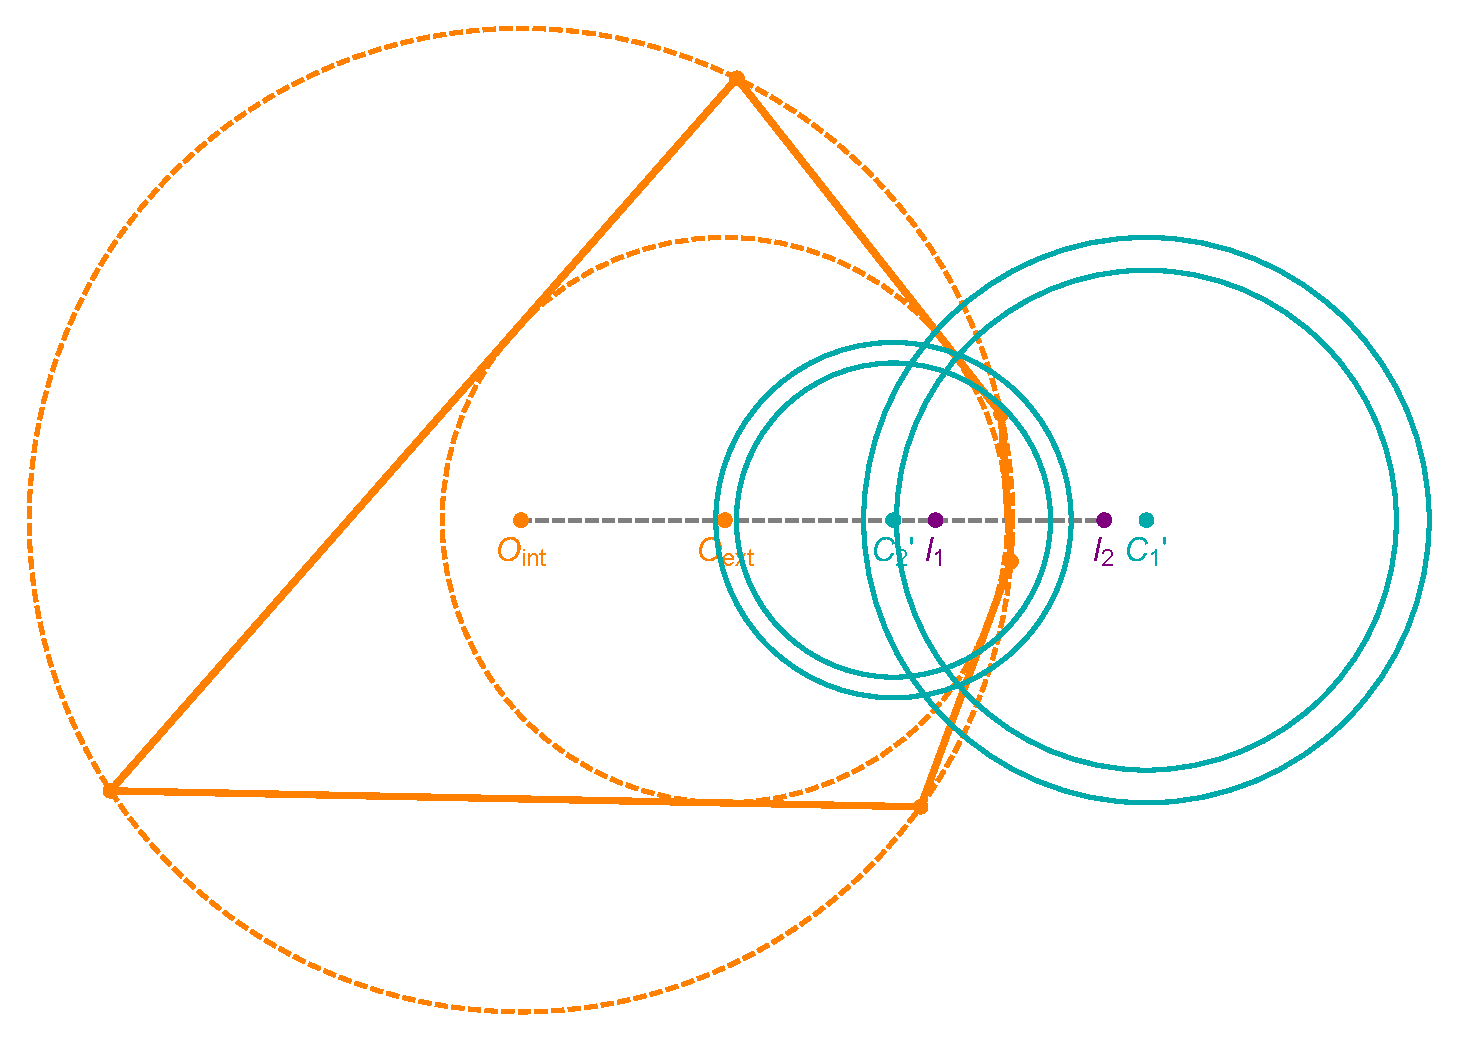
\includegraphics[width=.9\textwidth]{pics/0015_bicentric_with_concentric_pair.pdf}
%    \caption{A bicentric polygon (solid orange), interscribed between circles (dashed orange) centered on $O_{int}$ and $O_{ext}$. Also shown are the limiting points $\ell_1$ and $\ell_2$ as well as the two concentric pairs of circles (light blue) obtained by inverting the original circles wrt to unit circles centered at the the $\ell_i$. Note both concentric pairs have the same ratio of radii.
%    \label{fig:bicentric-with-concentric-pair}
%\end{figure}

\textbf{Main Results:}
Though the bicentric family was much studied in the last 200 years, interactive experimentation with their dynamic geometry has led us to detect and prove a few new curious facts, perhaps known to the giants of the XIX century but never jotted down.

\begin{itemize}
    \item \cref{thm:bicentric-sum}: The sum of the cosines of bicentric polygons is invariant over the family. This mirrors an invariant recently proved for elliptic billiard N-periodics \cite{reznik2020-intelligencer,garcia2020-new-properties,akopyan2020-invariants,bialy2020-invariants}.
    \item  \cref{thm:bicentric-pedal-perimeter} The perimeter of pedal polygons of the bicentrics with respect to its limiting points is invariant; see \cref{fig:confocal}. Notice this too mirrors perimeter invariance of elliptic billiard N-periodics.
    \item \cref{cor:inv-per}: Bicentric pedals with respect to a limiting point are identical to the inversion of billiard N-periodics with respect to a focus, therefore the latter also conserves perimeter. In fact it was this surprising observation (see this \href{https://youtu.be/wkstGKq5jOo}{Video}) that prompted the current article.
    \item \cref{conj:limiting-sum-cosines}: Experiments show that the two limiting pedal polygons also conserve their sum of cosines, except for  the case of the $N=4$ pedal with respect to $\ell_1$.
\end{itemize}



%\begin{figure}
%    \centering
%    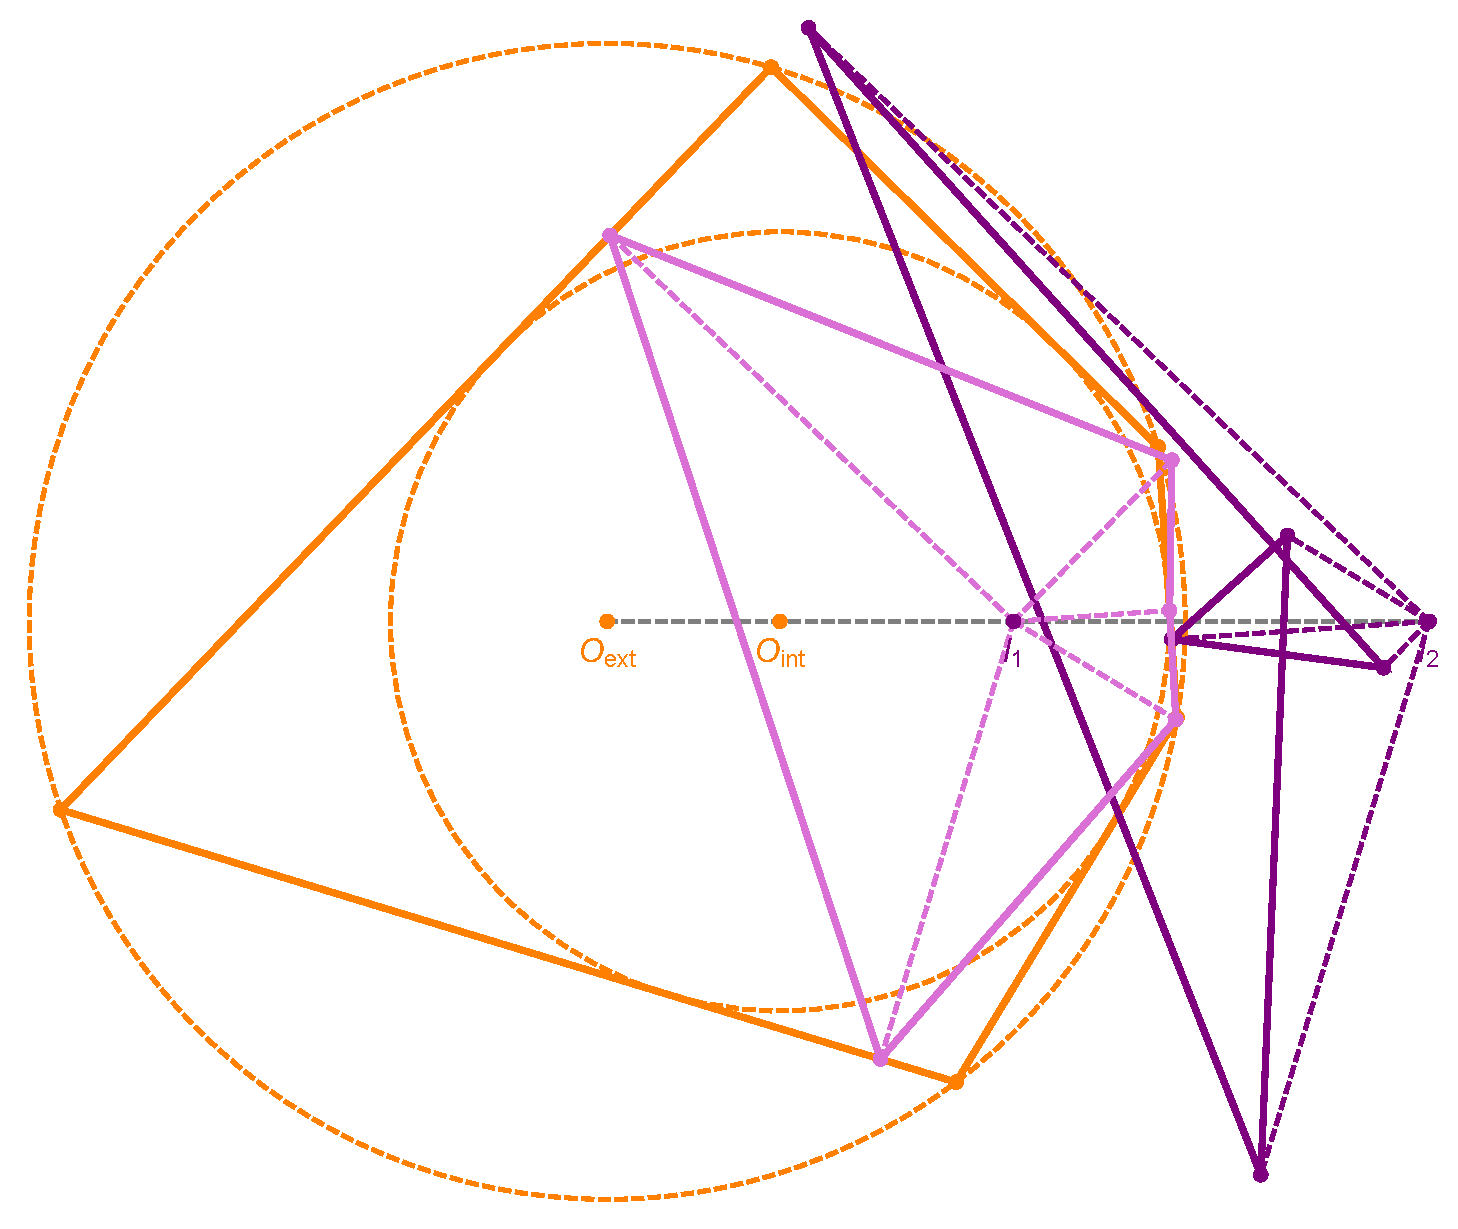
\includegraphics[width=.9\textwidth]{pics/0020_two_pedals.pdf}
%    \caption{The two constant-perimeter pedal polygons (pink and purple) whose vertices are at the feet of perpendiculars dropped from $\ell_1$ and $\ell_2$ respectively, onto the sidelines of the bicentric family (solid orange).}
%    \label{fig:two-pedals}
%\end{f

%\begin{figure}
%    \centering
%    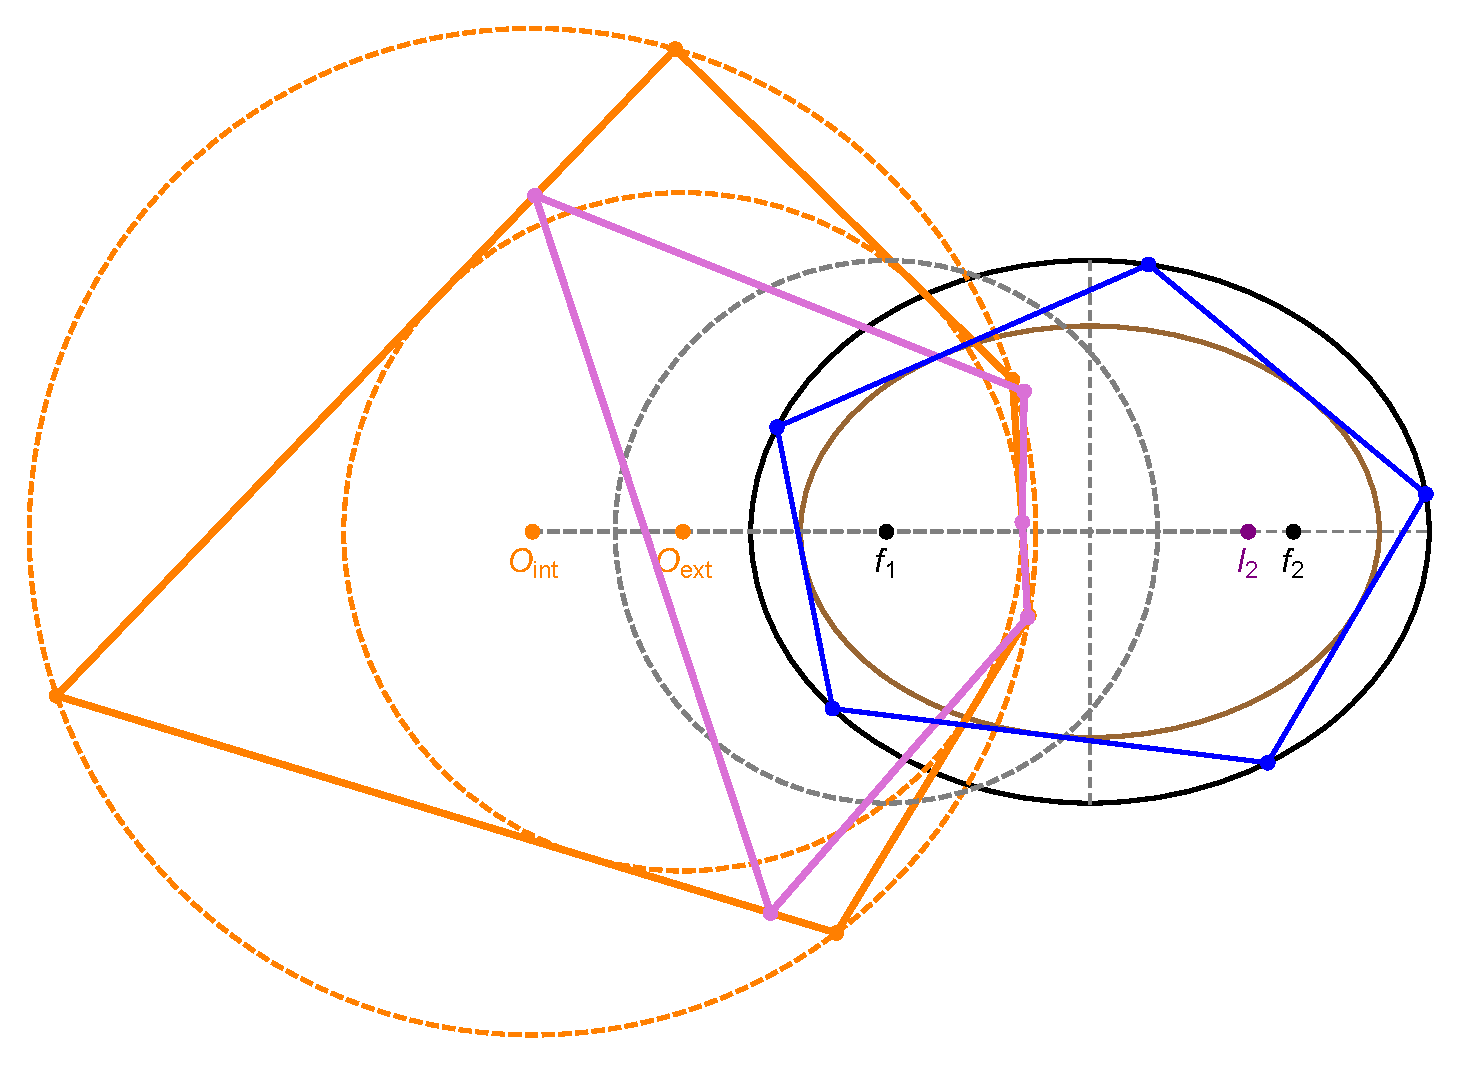
\includegraphics[width=.9\textwidth]{pics/0035_basic_billiard_plot.pdf}
%    \caption{The $f_1$-inversive polygon (pink) is the pedal polygon of a bicentric N-periodic (orange) with respect to the limiting point coinciding with $f_1$.}
%    \label{fig:basic-confocal}
%\end{figure}


%\begin{figure}
%    \centering
%    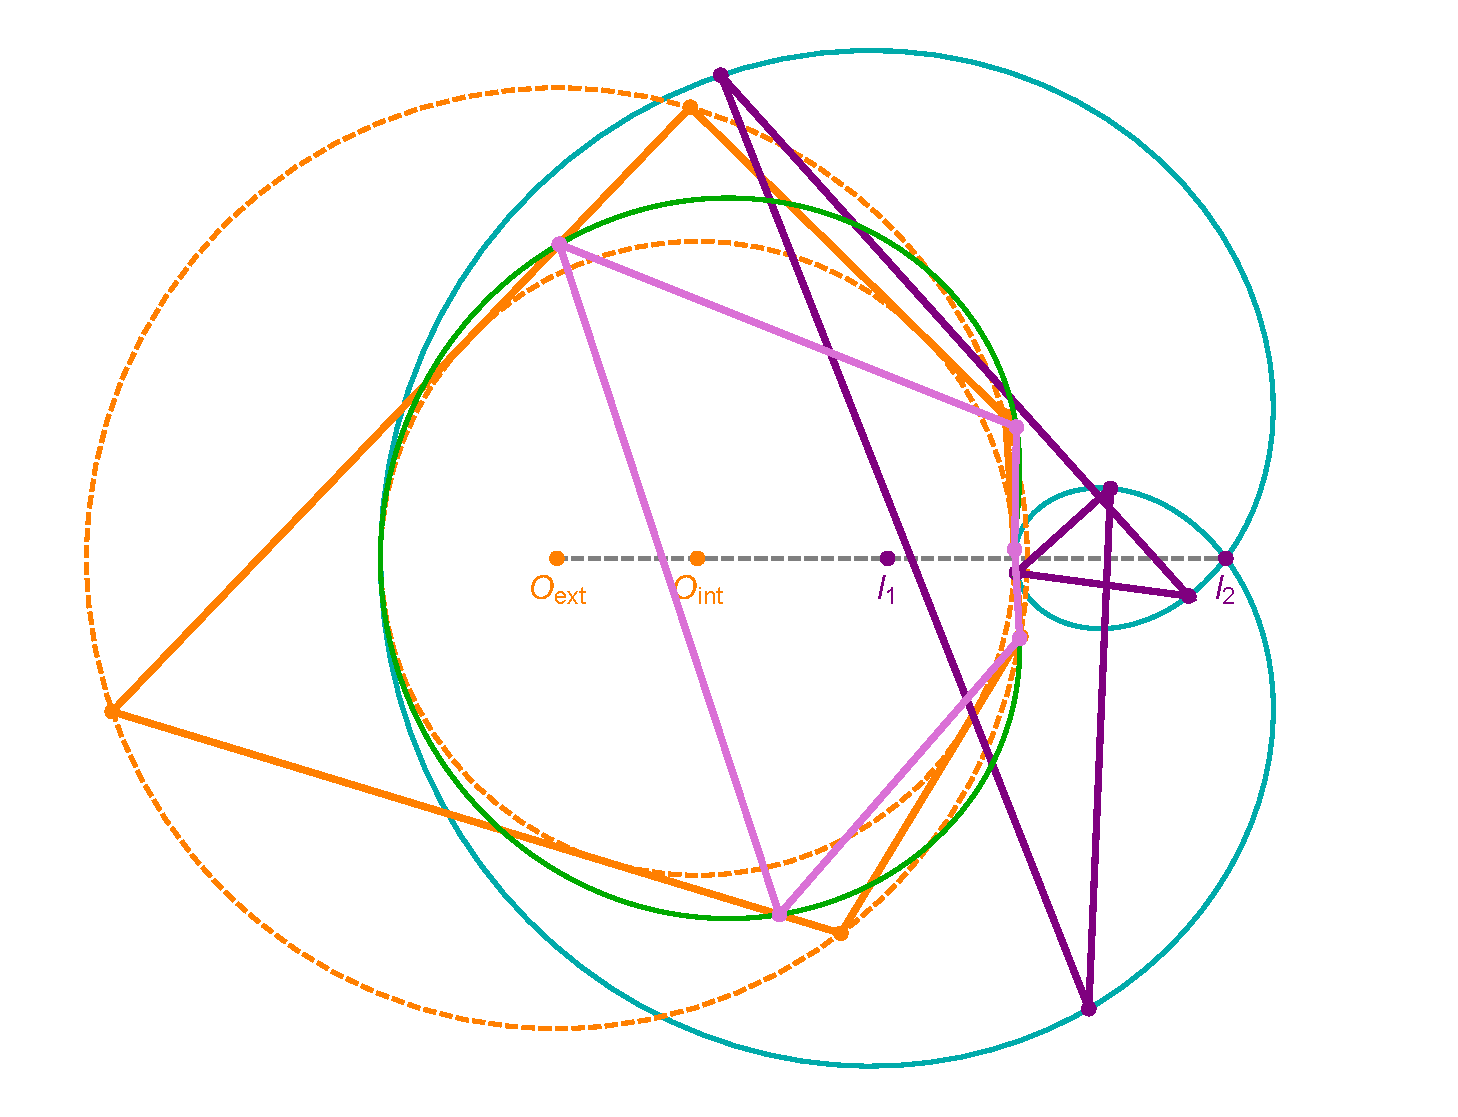
\includegraphics[width=.9\textwidth]{pics/0030_limacons.pdf}
%    \caption{Over the bicentric family (solid orange), the constant-perimeter $\ell_1$- and $\ell_2$ pedals (pink and purple) are inscribed in two separate Limaçons of Pascal: the former (green) is loopless, while the latter (aquamarine) has a loop passing through $\ell_2$.}
%    \label{fig:limacons}
%\end{figure}

\subsection*{Article Structure}
In \cref{sec:jacobi}, we review Jacobi's parametrization for bicentric polygons. We then use it to obtain expressions in terms of Jacobi elliptic functions for each of the above invariants, see \cref{sec:bicentric-sum-of-cosines,sec:pedal-perimeter}. \cref{sec:five-polys} paints a unified view of the five polygon families mentioned herein. A list of illustrative videos appear in \cref{sec:videos}. 

Details of polar and pedal transformations are covered in \cref{app:polar-pedal}. The parameters for a pair of confocal ellipses (or hyperbolas) which are the polar image of the bicentric pair are given in \cref{app:bicentric-to-confocal}. Conversely, the parameters for a bicentric pair which is the polar image of confocal ellipses are given in
\cref{app:confocal-to-bicentric}. In \cref{app:bicentric-vertices-n34} we provide elementary parametrizations for the vertices of $N=3$ and $N=4$ bicentric polygons. In \cref{app:pedal-perimeters-n34} we provide explicit expressions of their perimeters and sums of cosines as well as curious properties thereof.

%\begin{figure}
%    \centering
%    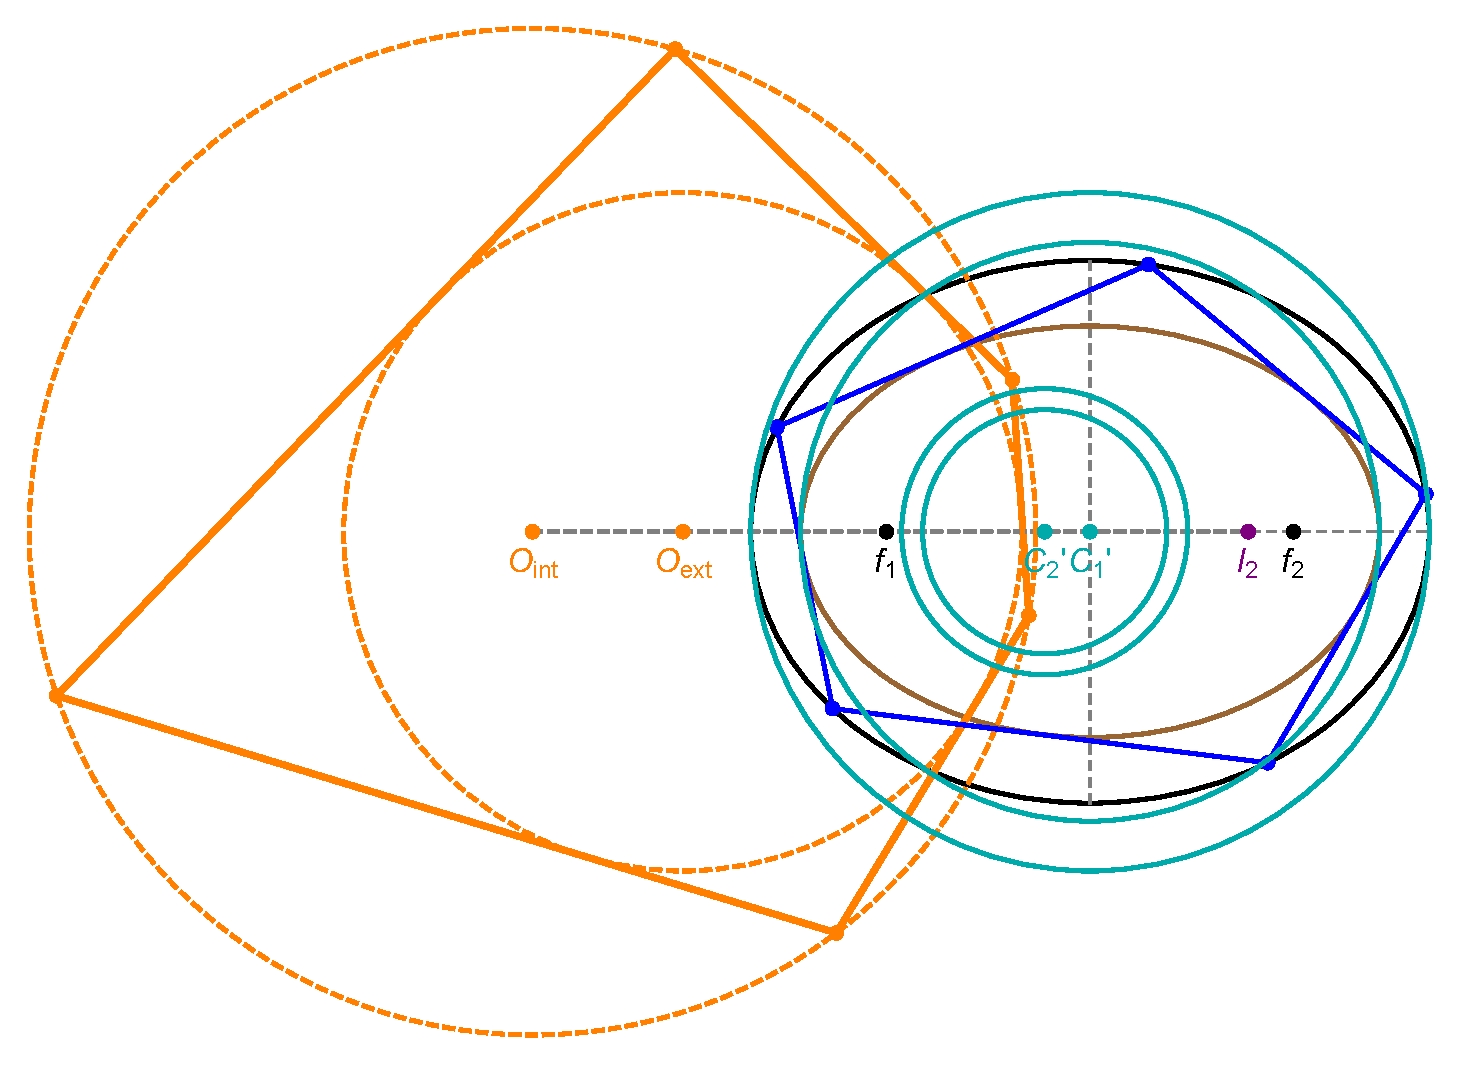
\includegraphics[width=.9\textwidth]{pics/0045_concentric_pairs_and_billiard.pdf}
%    \caption{The bicentric family (orange) is the polar image of billiard N-periodics (blue). These are Poncelet polygons interscribed between two confocal ellipses (black and brown). In particular one of the foci $f_1$ coincides with a first ``focal'' limiting point. In this configuration, the other one, $l_2$, appears in the positive x-axis. Also shown are the two pairs of concentric circles (aquamarine) centered on $C_1'$ and $C_2'$ which are inversive images of the bicentric circles wrt to unit radius circles centered at $f_1$ and $l_2$. Notice one of the pairs is centered at the billiard center, with a first (resp. second) circle circumscribing the billiard (resp. caustic).}
%    \label{fig:billiard-and-concentric-circles}
%\end{figure}


\subsection*{Related Work}

A few experimental of our experimental conjectures for elliptic billiard N-periodic invariants \cite{reznik2020-intelligencer,garcia2020-new-properties} have been proved: (i) invariant sum of cosines and (ii) invariant product of outer polygon cosines \cite{akopyan2020-invariants,bialy2020-invariants}, and (iii) invariant outer-to-orbit area ratio (for odd N) \cite{caliz2020-area-product}. Dozens of other conjectured invariants appear in \cite{reznik2021-fifty}.